\documentclass[12pt,letterpaper]{article}
\usepackage{graphicx,textcomp}
\usepackage{natbib}
\usepackage{setspace}
\usepackage{fullpage}
\usepackage{color}
\usepackage[reqno]{amsmath}
\usepackage{amsthm}
\usepackage{fancyvrb}
\usepackage{amssymb,enumerate}
\usepackage[all]{xy}
\usepackage{endnotes}
\usepackage{lscape}
\newtheorem{com}{Comment}
\usepackage{float}
\usepackage{hyperref}
\newtheorem{lem} {Lemma}
\newtheorem{prop}{Proposition}
\newtheorem{thm}{Theorem}
\newtheorem{defn}{Definition}
\newtheorem{cor}{Corollary}
\newtheorem{obs}{Observation}
\usepackage[compact]{titlesec}
\usepackage{dcolumn}
\usepackage{tikz}
\usetikzlibrary{arrows}
\usepackage{multirow}
\usepackage{xcolor}
\newcolumntype{.}{D{.}{.}{-1}}
\newcolumntype{d}[1]{D{.}{.}{#1}}
\definecolor{light-gray}{gray}{0.65}
\usepackage{url}
\usepackage{listings}
\usepackage{color}

\definecolor{codegreen}{rgb}{0,0.6,0}
\definecolor{codegray}{rgb}{0.5,0.5,0.5}
\definecolor{codepurple}{rgb}{0.58,0,0.82}
\definecolor{backcolour}{rgb}{0.95,0.95,0.92}

\lstdefinestyle{mystyle}{
	backgroundcolor=\color{backcolour},   
	commentstyle=\color{codegreen},
	keywordstyle=\color{magenta},
	numberstyle=\tiny\color{codegray},
	stringstyle=\color{codepurple},
	basicstyle=\footnotesize,
	breakatwhitespace=false,         
	breaklines=true,                 
	captionpos=b,                    
	keepspaces=true,                 
	numbers=left,                    
	numbersep=5pt,                  
	showspaces=false,                
	showstringspaces=false,
	showtabs=false,                  
	tabsize=2
}
\lstset{style=mystyle}
\newcommand{\Sref}[1]{Section~\ref{#1}}
\newtheorem{hyp}{Hypothesis}

\title{Problem Set 2}
\date{Due: October 14, 2024}
\author{Applied Stats/Quant Methods 1}

\begin{document}
	\maketitle
	\section*{Instructions}
\begin{itemize}
	\item Please show your work! You may lose points by simply writing in the answer. If the problem requires you to execute commands in \texttt{R}, please include the code you used to get your answers. Please also include the \texttt{.R} file that contains your code. If you are not sure if work needs to be shown for a particular problem, please ask.
	\item Your homework should be submitted electronically on GitHub.
	\item This problem set is due before 23:59 on Monday October 14, 2024. No late assignments will be accepted.

\end{itemize}

	
	\vspace{.5cm}
	\section*{Question 1: Political Science}
		\vspace{.25cm}
	The following table was created using the data from a study run in a major Latin American city.\footnote{Fried, Lagunes, and Venkataramani (2010). ``Corruption and Inequality at the Crossroad: A Multimethod Study of Bribery and Discrimination in Latin America. \textit{Latin American Research Review}. 45 (1): 76-97.} As part of the experimental treatment in the study, one employee of the research team was chosen to make illegal left turns across traffic to draw the attention of the police officers on shift. Two employee drivers were upper class, two were lower class drivers, and the identity of the driver was randomly assigned per encounter. The researchers were interested in whether officers were more or less likely to solicit a bribe from drivers depending on their class (officers use phrases like, ``We can solve this the easy way'' to draw a bribe). The table below shows the resulting data.

\newpage
\begin{table}[h!]
	\centering
	\begin{tabular}{l | c c c }
		& Not Stopped & Bribe requested & Stopped/given warning \\
		\\[-1.8ex] 
		\hline \\[-1.8ex]
		Upper class & 14 & 6 & 7 \\
		Lower class & 7 & 7 & 1 \\
		\hline
	\end{tabular}
\end{table}

\begin{enumerate}
	
	\item [(a)]
	Calculate the $\chi^2$ test statistic by hand/manually (even better if you can do "by hand" in \texttt{R}).\\

	To calculate the Chi-squared statistic by hand, we first have to calculate the expected values for each respective observation. This can be found by dividing the row sum by the grand total and multiplying this by the column total.
	\lstinputlisting[language=R, firstline=38, lastline=58]{PS02_FOS.R}  
	\begin{verbatim}
		     [,1]     [,2]     [,3]
		[1,] 13.5 8.357143 5.142857
		[2,]  7.5 4.642857 2.857143
	\end{verbatim}
	
	From here, the Chi-squared statistic is given by taking the average of each squared difference between the observed and expected values divided by the expected values.
	
	\lstinputlisting[language=R, firstline=61, lastline=62]{PS02_FOS.R}  
	\begin{verbatim}
		[1] 3.791168
	\end{verbatim}
	
		
	\vspace{2cm}
	\item [(b)]
	Now calculate the p-value from the test statistic you just created (in \texttt{R}).\footnote{Remember frequency should be $>$ 5 for all cells, but let's calculate the p-value here anyway.}  What do you conclude if $\alpha = 0.1$?\\
	
	To calculate the associated p-value for our test-statistic, we consult the Chi-squared PDF with the appropirate degrees of freedom
	
	\lstinputlisting[language=R, firstline=68, lastline=69]{PS02_FOS.R}  
	\begin{verbatim}
		[1] 0.2849151
	\end{verbatim}
	
	We can conclude that even with a non-stringent alpha of 0.1, we cannot reject the null hypothesis that the groups are independent.
	
	\newpage
	\item [(c)] Calculate the standardized residuals for each cell and put them in the table below.
	\vspace{1cm}
	
	To calculate the standardised/adjusted residuals we convert the difference between the expected and observed to units of standard error. For the Chi-squared distribution, the standard error is the square root of the product of each respective expected value by 1 minus the proportions for both the row and column totals
	
	\lstinputlisting[language=R, firstline=77, lastline=97]{PS02_FOS.R}  
	
	\begin{table}[h]
		\centering
		\begin{tabular}{l | c c c }
			& Not Stopped & Bribe requested & Stopped/given warning \\
			\\[-1.8ex] 
			\hline \\[-1.8ex]
			Upper class  &  0.32 &  -1.64  & 1.52  \\  
			\\
			Lower class &  -0.32 &  1.64  & -1.52  \\
			
		\end{tabular}
	\end{table}
	
	
	\vspace{7cm}
	\item [(d)] How might the standardized residuals help you interpret the results?  
	
	These results are incorrect. The first indication of this is that the matrix is symmetric. Having spent the weekend trouble-shooting this, I know that the issue is with the loop before the residuals are calculated and not with the final simple matrix subtraction and division. Here is the standard error matrix after the loop has run:
	
	\begin{verbatim}
		         [,1]    [,2]     [,3]
		[1,] 1.552648 1.43557 1.219377
		[2,] 1.552648 1.43557 1.219377
	\end{verbatim}
 		
 	This suggests the issue may be with the row indexing, either overwriting the results of the first row over the second or simply computing the first row twice. I have written i-j loops in MATLAB but it has been some time. I broke the process down into two separate loops, like what I used for question 1a. I noticed that some values were correct by comparing these results to calculations of the standard error done by hand, and therefore suspect that standard error function may be the source of the error or a second error.
 	
 	\lstinputlisting[language=R, firstline=101, lastline=109]{PS02_FOS.R}  
 	
 	I also tried defining a specific standard error function and then using the apply function, but this proved more of an issue. I suspect loops were not necessary, and the entire procedure could be done with apply.  I could also have just installed a package that calculated the residuals, but that would have been no fun! ChatGPT was useless and I should simply have started earlier and discussed the issue during office hours. Any suggestions, either for spotting the error in the single loops, the nested loop, or for using the apply function, would be very much appreciated! 
 	
 	Lastly, in general the residuals help us interpret the distance between the observed and expected values in terms of standard error units rather than raw values.
 	 	
 			
\end{enumerate}
\newpage

\section*{Question 2: Economics}
Chattopadhyay and Duflo were interested in whether women promote different policies than men.\footnote{Chattopadhyay and Duflo. (2004). ``Women as Policy Makers: Evidence from a Randomized Policy Experiment in India. \textit{Econometrica}. 72 (5), 1409-1443.} Answering this question with observational data is pretty difficult due to potential confounding problems (e.g. the districts that choose female politicians are likely to systematically differ in other aspects too). Hence, they exploit a randomized policy experiment in India, where since the mid-1990s, $\frac{1}{3}$ of village council heads have been randomly reserved for women. A subset of the data from West Bengal can be found at the following link: \url{https://raw.githubusercontent.com/kosukeimai/qss/master/PREDICTION/women.csv}\\

\noindent Each observation in the data set represents a village and there are two villages associated with one GP (i.e. a level of government is called "GP"). Figure~\ref{fig:women_desc} below shows the names and descriptions of the variables in the dataset. The authors hypothesize that female politicians are more likely to support policies female voters want. Researchers found that more women complain about the quality of drinking water than men. You need to estimate the effect of the reservation policy on the number of new or repaired drinking water facilities in the villages.
\vspace{.5cm}
\begin{figure}[h!]
	\caption{\footnotesize{Names and description of variables from Chattopadhyay and Duflo (2004).}}
	\vspace{.5cm}
	\centering
	\label{fig:women_desc}
	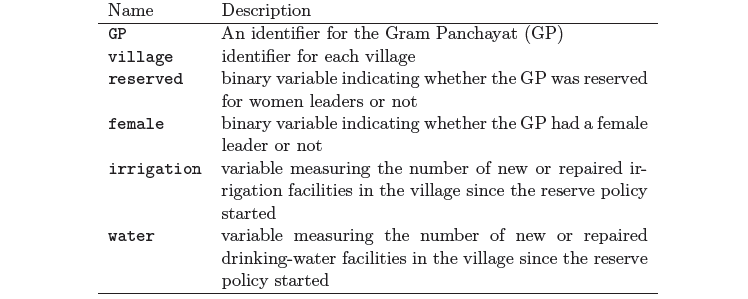
\includegraphics[width=1.1\textwidth]{women_desc.png}
\end{figure}		

\newpage
\begin{enumerate}
	\item [(a)] State a null and alternative (two-tailed) hypothesis. 
	
	The null hypothesis here is that there is no correlation between male and female representatives (input variable) and the number of repairs to/new water facilities (response variable). The alternative hypothesis is that there does exist a correlation. As a two-sided test we are not testing whether there is an increase in response variable. This can be summarised as \textit{H0: B-hat = 0 and Ha: B-hat != 0}
	
	\vspace{2cm}
	\item [(b)] Run a bivariate regression to test this hypothesis in \texttt{R} (include your code!).
	
	\lstinputlisting[language=R, firstline = 135 lastline = 172]{PS02_FOS.R} 
	
	The results of the linear regression run on the merged response variables, and the correlation test, are as follows
	
\begin{verbatim}
Coefficients:
(Intercept)       female  
14.813        7.864  
	
	
	Pearson's product-moment correlation

data:  df_raw$female and df_raw$water
t = 2.0491, df = 320, p-value = 0.04126
alternative hypothesis: true correlation is not equal to 0
95 percent confidence interval:
0.004563936 0.220363186
sample estimates:
cor 
0.1138057
\end{verbatim}


	
\begin{figure}[h!]
		\caption{\footnotesize{Basic plot of binary input variable regression}}
		\label{regression.png}
		\includegraphics[width=1.1\textwidth]{regression.png}
\end{figure}			
	
\end{enumerate}	



\begin{enumerate}
	\newpage
	\item [(c)] Interpret the coefficient estimate for reservation policy. 
	
	The value we get for the correlation coefficient is 0.11, with a p-value of 0.04. Thus, if we were conducting a hypothesis test with an alpha of 0.05, we would just about be able to reject the null hypothesis that, specifically, there is no statistically significant effect of the reservation policity on number of new or repaired water facilities in the sample provided. The alternative hypothesis, that there is an effect of the reservation policy, could be accepted at this alpha threshold. The spread around this p-value, as measured by the 95 percent confidence interval is quite large however, which we could interpreted as noisy data and would lend caution to making strong claims about just how effective the policy has been.
	
	The data can also be aggregated to look at the merged response variables, namely changes to both irrigation and water facilities, which dampens the correlation and suggests specificity of the policy to water-drinking facilities rather than a general effect on water-facilities including drinking water and irrigation.
	
\end{enumerate}

\end{document}
